%--------------------
% Packages
% -------------------
\documentclass[11pt,a4paper]{article}
\usepackage[utf8x]{inputenc}
\usepackage[T1]{fontenc}
\usepackage{mathptmx} % Use Times Font
\usepackage[pdftex]{graphicx} % Required for including pictures
% \usepackage[pdftex,linkcolor=black,pdfborder={0 0 0}]{hyperref} % Format links for pdf
\usepackage{calc} % To reset the counter in the document after title page
\usepackage{enumitem} % Includes lists
\usepackage{csquotes} % Exercise as quotes
\usepackage{amsmath} % For using "equation*" 
\usepackage{nicefrac} % For in-line fractions

\setcounter{equation}{0}% How to reset equation counter

\frenchspacing % No double spacing between sentences
\linespread{1.2} % Set linespace
\usepackage[a4paper, lmargin=0.1666\paperwidth, rmargin=0.1666\paperwidth, tmargin=0.1111\paperheight, bmargin=0.1111\paperheight]{geometry} %margins
%\usepackage{parskip}

\usepackage[all]{nowidow} % Tries to remove widows
\usepackage[protrusion=true,expansion=true]{microtype} % Improves typography, load after fontpackage is selected
%-----------------------
% Set pdf information and add title, fill in the fields
%-----------------------
% \hypersetup{ 	
% pdfsubject = {Nano-Optics},
% pdftitle = {Assignment 1},
% pdfauthor = {Vlad Tkachuk}
% }

%-----------------------
% Begin document
%-----------------------
\begin{document} 

\section{Theory}
\subsection*{Exercise 1}


\begin{figure}[ht]
   \centering
    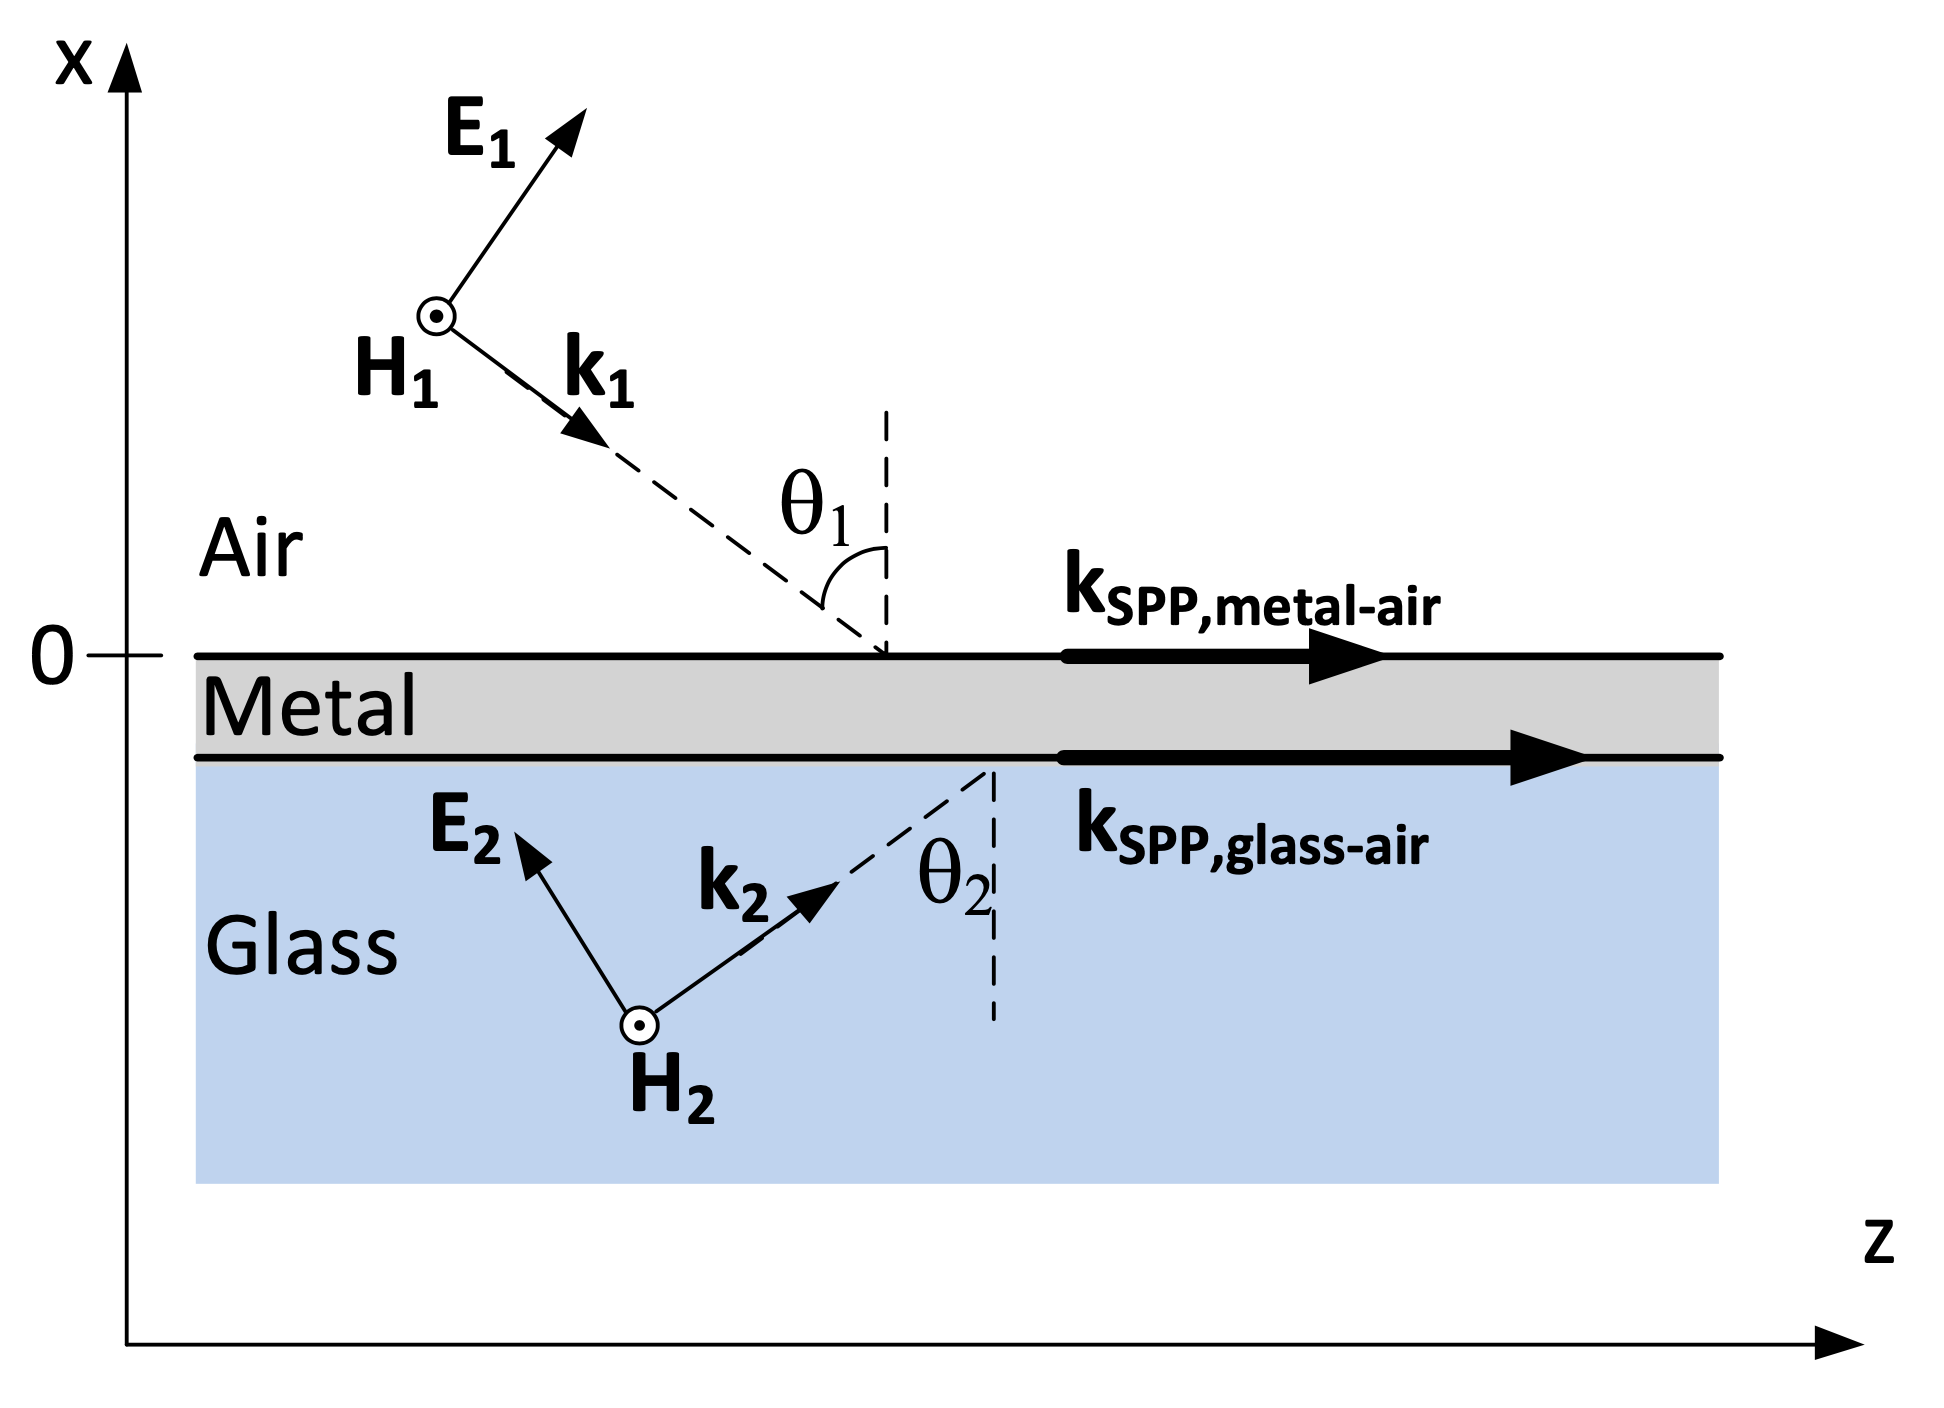
\includegraphics[width=0.45\textwidth]{fig_0.png}
    \caption{}
    \label{fig:fig0}
\end{figure}

\begin{figure}[ht]
   \centering
    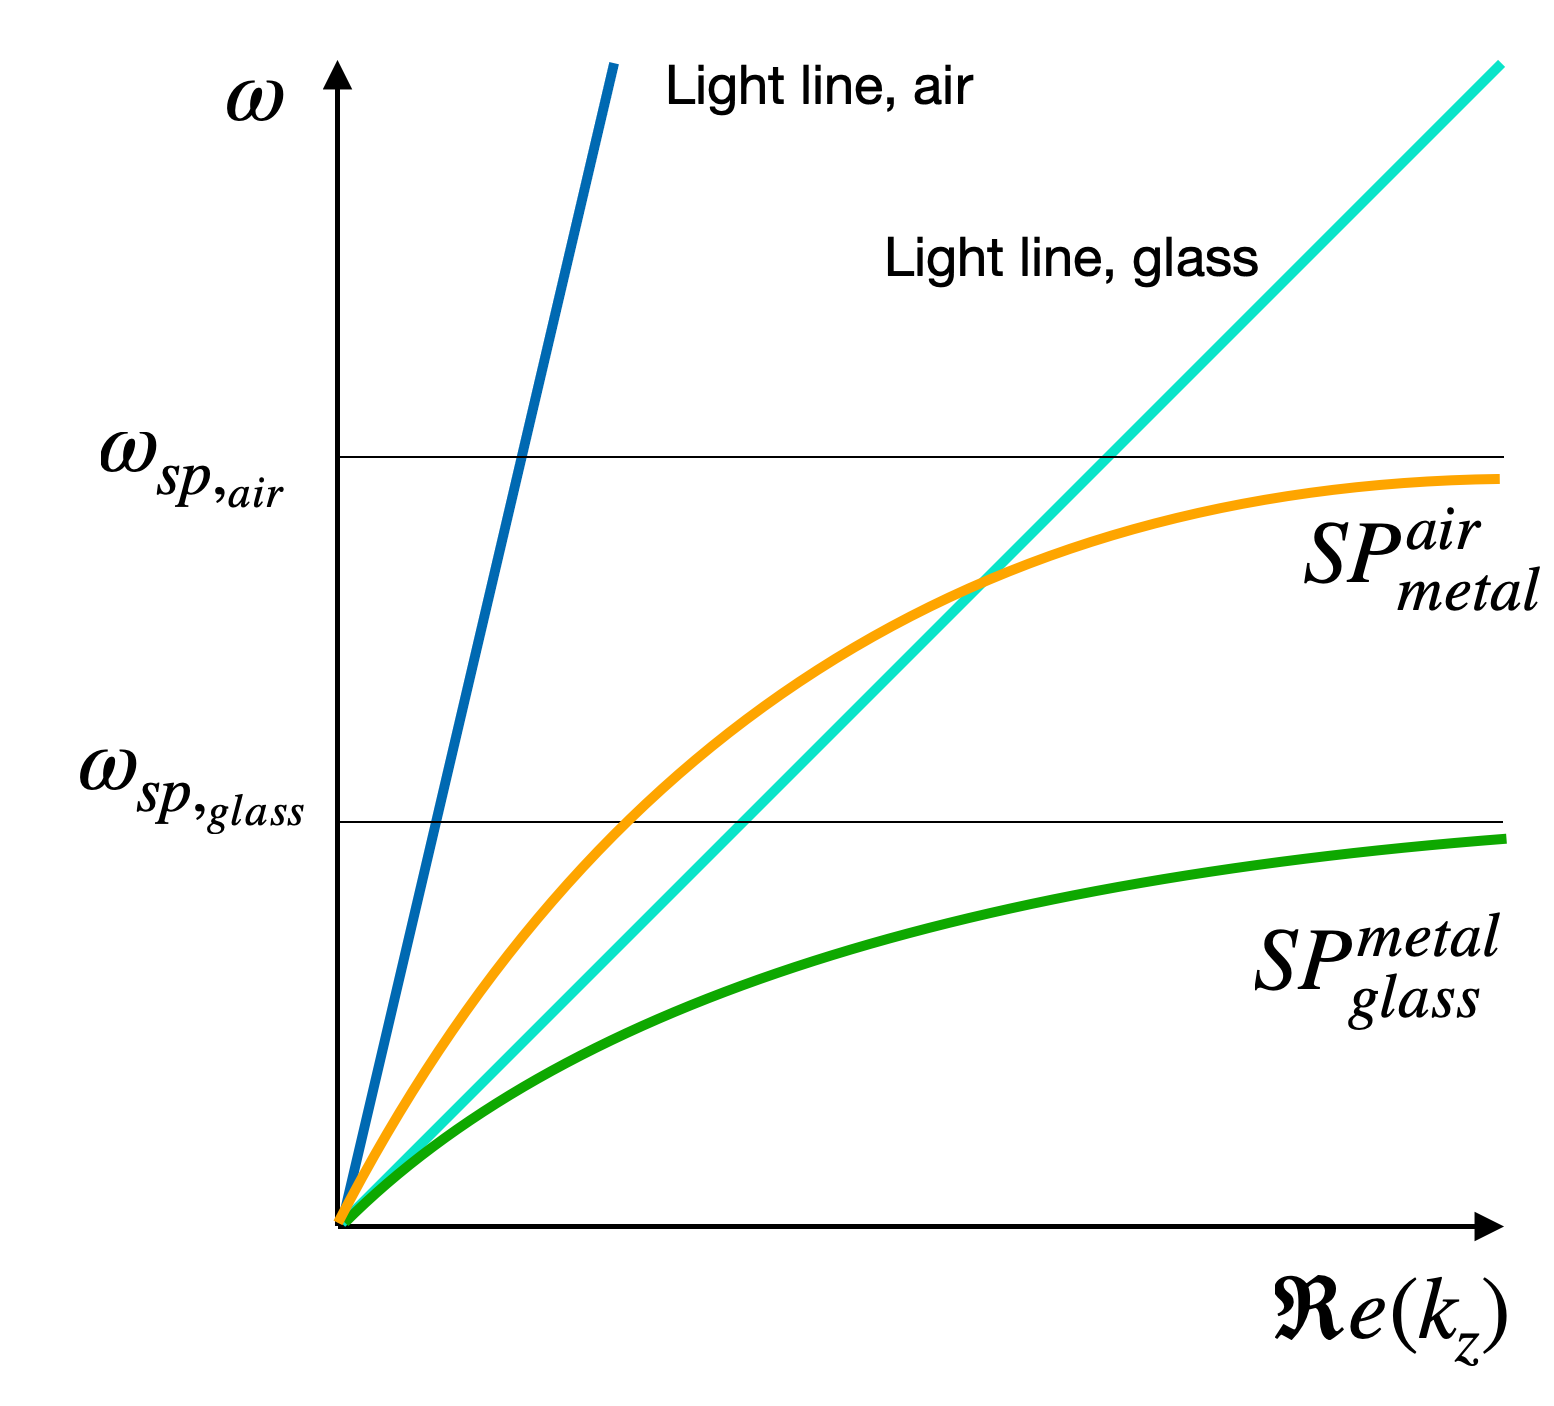
\includegraphics[width=0.45\textwidth]{fig_1.png}
    \caption{Dispersion relation of the surface plasmons.}
    \label{fig:fig1}
\end{figure}



\textbf{a. }Consider the structure depicted in Figure~\ref{fig:fig0}. It consists of a glass (SiO\textsubscript{2}) substrate with a layer of ideal metal deposited on it. The thickness of this metal layer is thick enough to permit the propagation of a surface plasmon polariton at each dielectric-metal interface (i.e., metal-air and metal-glass interfaces). The propagation vectors for these two surface plasmons have been shown in the figure. The thickness of the metal layer is, however, sufficiently thin to permit exciting any of the two surface plasmons when an electromagnetic field is incident upon the film from one of its sides.

\begin{displayquote}
\textbf{1.}  Plot the dispersion relation of an electromagnetic field
propagating through the air (eg., Field 1 in Figure 2).
\end{displayquote}
From the definition of dispersion relation, for light line in air: 

\begin{equation}
    \frac{\omega}{k}\Big|_{air}=v_{air}=\frac{c}{n_{air}}=\frac{c}{\sqrt{\varepsilon_{air}}}
\end{equation}


\begin{displayquote}
\textbf{2.}  In the same graph, plot the dispersion relation of an electromagnetic field propagating through the glass (eg., Field 2 in Figure 2).
\end{displayquote}

Analogically, for glass:

\begin{equation}
     \frac{\omega}{k}\Big|_{glass}=v_{glass}=\frac{c}{n_{glass}}=\frac{c}{\sqrt{\varepsilon_{glass}}}
\end{equation}

\begin{displayquote}
\textbf{3.}  Plot now the dispersion relation of the surface plasmon polariton traveling in the air/metal interface.
\end{displayquote}
Dispersion relation for dielectric-metal interface ($\varepsilon_d, \varepsilon_m$ correspondingly) can be expressed as:
\begin{equation}
    k_z=\frac{\omega}{c}\sqrt{\frac{\varepsilon_m \varepsilon_d}{\varepsilon_m + \varepsilon_d}} \Leftrightarrow k_z = \frac{\omega}{c}\sqrt{\frac{(\omega^2-\omega^2_p) \varepsilon_d}{(1+\varepsilon_d) \omega^2 - \omega^2_p}}
\end{equation}

\begin{displayquote}
    \textbf{4.}  Indicating what happens for the SPP wavelength (compare with its
wavelength in vacuum) at very small $\omega$ and at the resonance frequency ($\omega_{sp}$). Note that you can explain it based on the expression of the dispersion relation of the bound mode at that interface for very small frequencies and for frequencies close to the resonance.
\end{displayquote}
At very low frequency, dispersion relation of SPP tends to light line:
\begin{equation}
    \omega \to 0: \; k_z=\frac{\omega}{c} \lim_{\varepsilon_m \to -\infty} \sqrt{\frac{\varepsilon_m \varepsilon_d}{\varepsilon_m + \varepsilon_d}} \approx \frac{\omega}{c} \sqrt{\varepsilon_d}
\end{equation}

For very large wavevector, at resonance frequency:

\begin{equation}
    \varepsilon_m \to - \varepsilon_d, \; k_z \to \infty, \; \omega \equiv \omega_{sp} = \frac{\omega_p}{\sqrt{1+\varepsilon_d}}
\end{equation}

\begin{displayquote}
    \textbf{5.}  Indicate at which frequency the resonance takes place in the plot. 
    \end{displayquote}

    There will be resonance at $\omega_{sp}$.
    
    \begin{displayquote}
    \textbf{6.}  Do the same for the surface plasmon polariton traveling in the
glass/metal interface.
\end{displayquote}
The graphs would look similar. The only factual difference is that $\varepsilon_d$ now stands for glass. This means the line and curve are more inclined towards $k_z$-axis.

\begin{displayquote}
    \textbf{7.}  Indicate the resonance frequencies ($\omega_{sp}$) relation to the plasmon frequency ($\omega_p$)
\end{displayquote}
For simple Drude model,

\begin{equation}
    \omega_{sp} = \frac{\omega_p}{\sqrt{1+\varepsilon_d}}
\end{equation}

For modified Drude model, contribution of bound electrons ($\varepsilon_{\infty}$)  is included:
\begin{equation}
      \omega_{sp} = \frac{\omega_p}{\sqrt{\varepsilon_{\infty}+\varepsilon_d}}
\end{equation}

\textbf{b. }Remember that in order to achieve coupling between two waves, phase matching needs to be accomplished (i.e., the propagation vectors should match).



\begin{displayquote}
     Show in the diagram that you have drawn in (a) under which conditions (i.e., for which range of $k_{SPP}$ vectors) coupling between the field propagating in free space through air and one (or two) of the surface plasmon polaritons will take place, if possible. Please, note that the angle of incidence, $\theta_1$, can be varied to achieve phase matching.
\end{displayquote}

Consider the wavevector of incident light from above, $k_1$. Then depending on the angle of incidence, $\theta_1$, $k_1 = \nicefrac{\omega}{c} \sin{\theta_1}$. Recall that the light line is described by $k_{l,air}=\nicefrac{\omega}{c}$, because in air, $\varepsilon_d=1$. It is then evident that for $\theta_1 < 90 \deg$, $k_1 < k_{l,air} < k_{sp}$, and to couple from air, the phase matching condition cannot be satisfied for plain geometry. If then additional wavevector is added, for example, by grating with wavevector $K$, such that $K = \nicefrac{2 \pi}{\Lambda}$, where $\Lambda$ is period of the grating, then the condition can be satisfied, provided $\pm k_{sp} = k_1 + mK, \; m = \pm 1, \; \pm 2, \; ...$ (Figure~\ref{fig:cond1}).


\begin{figure}[ht]
   \centering
    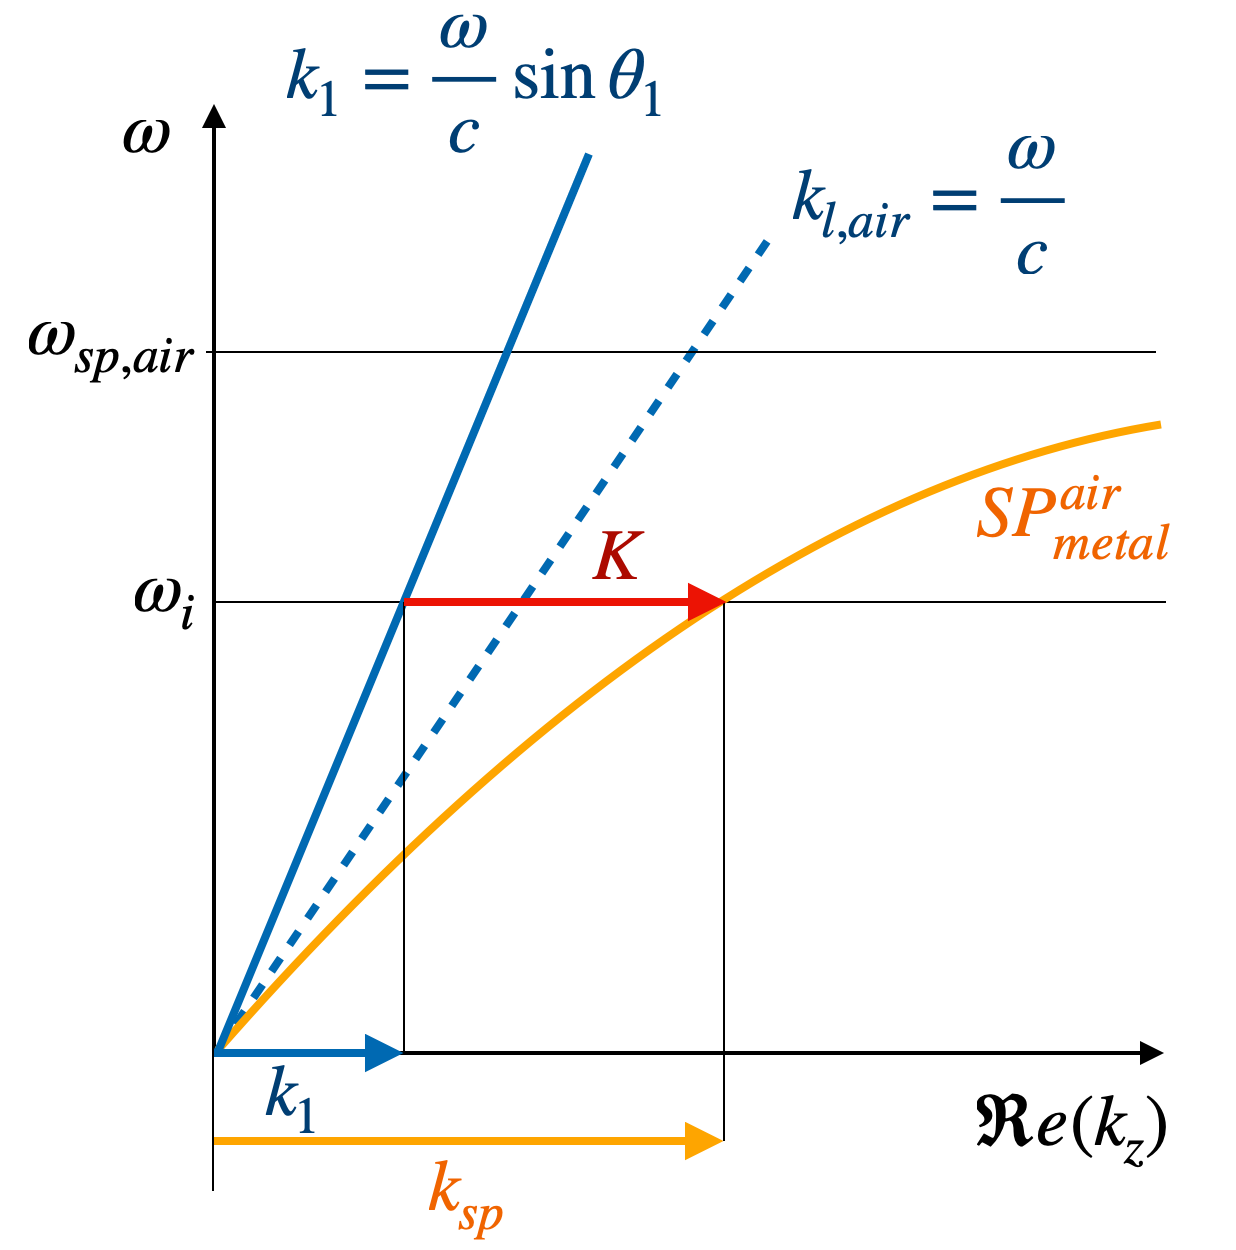
\includegraphics[width=0.45\textwidth]{cond1.png}
    \caption{Dispersion relation for coupling light from above (region 1) to SPP on air-metal interface.}
    \label{fig:cond1}
\end{figure}

Consider now the Field 2, incident from the glass:
\begin{displayquote}
    \textbf{2.} Show in the diagram which $\omega - k$ condition permits coupling of the field to one of the surface plasmon modes.
\end{displayquote}
In this case, illuminating glass with incident angle $\theta_2$, larger than the critical angle, will produce wavevector $k_2$ such that $k_{l,air} < k_2 < k_{l,glass}$, for which it is possible to satisfy the phase matching condition to couple to air-metal SPP, if the metal layer is thin enough (Figure~\ref{fig:cond2}). 

\begin{figure}[ht]
   \centering
    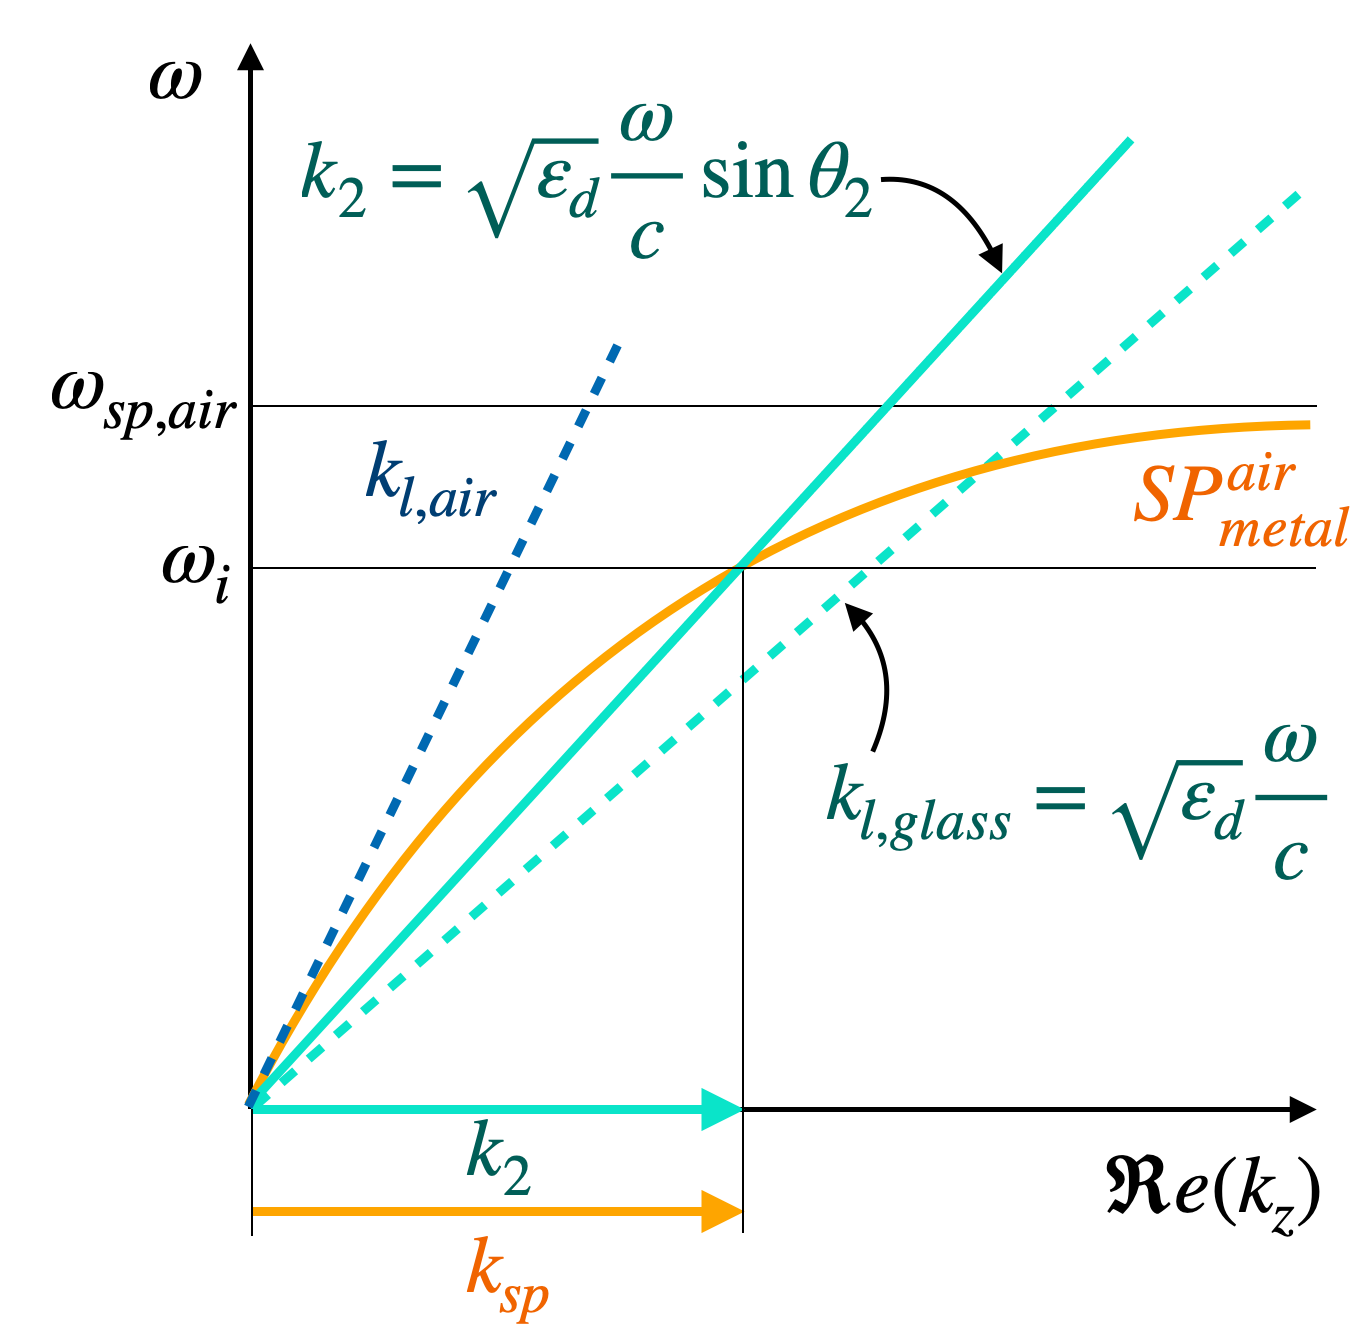
\includegraphics[width=0.45\textwidth]{cond2.png}
    \caption{Dispersion relation for coupling light from below (region 2) to SPP on air-metal interface.}
    \label{fig:cond2}
\end{figure}

If another dielectric layer with a refractive index larger than that of the glass is added below, the incident light through this dielectric layer can excite SPPs on the metal-glass interface at different incident angles.

\begin{displayquote}
\textbf{3.} What happens when you vary the angle of incidence?
\end{displayquote}
Varying the angle of incidence changes the magnitude of wavevector and, subsequently, will require a different wavelength of the incident light to match. 

\begin{displayquote}
\textbf{4.} To which range of $k_{SPP}$ of each of the two surface plasmons propagating in the structure could you couple?
\end{displayquote}
Theoretically any wavevector such that $k_{l,air} < k_2 < k_{l,glass}$. In practice, for complex $\varepsilon_m$ with non-zero real part, there will be a maximal supported value for $k_{SPP}$. Naturally, air-metal interface supports lower $k_{SPP}$ than that of metal-glass interface.

\subsection*{Exercise 2}

Consider a plasmonic mode propagating at the interface of gold ($\varepsilon_{r,gold} = −41.849 + j2$.) and aluminum oxide ($\varepsilon_{r,Al_2O_3} = 2.72$). The free space wavelength of the mode is 1 micrometer. Please, explain what you do to:

\begin{displayquote}
    \textbf{a.}  Calculate the propagation length of this waveguide. (the propagation length is defined as the 1/e value of the intensity)
\end{displayquote}

 Designate $\varepsilon_d, = \varepsilon_{r,Al_2O_3}  \; \varepsilon_m = \varepsilon_{r,gold}$.
The propagation of SPP at plane interface air-metal along the interface:

\begin{equation}
    \textbf{E}  = E_0 e^{j (k_z z - \omega t)}
\end{equation}
where wavevectors satisfy the relation:

\begin{equation}
    k^2_z+k^2_{d,m,x} = \varepsilon_{d,m} k^2
\end{equation}

for $k = \nicefrac{2 \pi}{\lambda}$, where $\lambda$ is vacuum wavelength. After applying the source-free assumption and the boundary conditions, insuring continuity, we obtain the dispersion relations. For wavevector component propagating along the interface: 

\begin{equation}
    k_z^2=\frac{\varepsilon_d \varepsilon_m}{\varepsilon_d + \varepsilon_m}k^2
\end{equation}

 Complex $\varepsilon_m$ leads to complex $k_z$. Because $\Im m (\varepsilon_{d,m}) \ll \Re e (\varepsilon_{d,m})$, we can see that in (8), $\Re e (k_z)$ determines SPP wavelength, and $\Im m (k_z)$ accounts for damping as it propagates along the interface:

 \begin{equation}
     \textbf{E}  = E_0 \big( e^{j (\Re e{(k_z)} z - \omega t)} e^{- \Im m{(k_z)} z}\big)
 \end{equation}

The definition of intensity:

\begin{equation}
    I = \sqrt{\frac{\varepsilon_0}{\mu_0}} |E(\omega)|^2 =\sqrt{\frac{\varepsilon_0}{\mu_0}} E_0^2 e^{-2 \Im m (k_z) z}
\end{equation}

The intensity at $z = 0$ is:

\begin{equation}
    I \big|_{z=0} = \sqrt{\frac{\varepsilon_0}{\mu_0}} E_0^2
\end{equation}

Using the definition of propagation length: 
\begin{equation}
    \frac{1}{e} I \big|_{z=0} =  I \big|_{z=L_{prop}}
\end{equation}

Then:
\begin{equation}
   \frac{1}{e} \sqrt{\frac{\varepsilon_0}{\mu_0}} E_0^2 = \sqrt{\frac{\varepsilon_0}{\mu_0}} E_0^2 e^{-2 \Im m (k_z) L_{prop}} \Rightarrow L_{prop}=\frac{1}{2 \Im m (k_z)}
\end{equation}

Finally,

\begin{equation}
    L_{prop}=\frac{1}{2 \Im m \big(\frac{2 \pi}{\lambda}\sqrt{\frac{\varepsilon_d \varepsilon_m}{\varepsilon_d + \varepsilon_m}}\big)} = 2.816 \cdot 10^{-5} \; [m]
\end{equation}


\begin{displayquote}
\textbf{b. } Calculate the penetration into the dielectric and into the metal (the penetration is defined as the 1/e value of the intensity).
\end{displayquote}

The normal component of wavevector:
\begin{equation}
    k_{d,m}^2=\frac{\varepsilon_{d,n}^2}{\varepsilon_d+\varepsilon_m} k^2
\end{equation}

And the same relation holds for depth of propagation in metal and dielectric as in (15):

\begin{equation}
     \delta_{d,m}=\frac{1}{2 \Im m (k_{d,m})}
\end{equation}

Hence:
\begin{equation}
    \delta_{d}=\frac{1}{2 \Im m \big(\frac{2 \pi}{\lambda}\sqrt{\frac{\varepsilon_d^2}{\varepsilon_d + \varepsilon_m}}\big)}= -1.832 \cdot 10^{-7} \; [m]
\end{equation}

\begin{equation}
    \delta_{m}=\frac{1}{2 \Im m \big(\frac{2 \pi}{\lambda}\sqrt{\frac{\varepsilon_m^2}{\varepsilon_d + \varepsilon_m}}\big)}= 1.189 \cdot 10^{-8} \; [m]
\end{equation}

Different sign of results in (19) and (20) confirm the expectation. The numerical result was calculated in Mathcad. 

\subsection{Exercise 3}

Demonstrate that, at very low frequencies ($\omega \ll \omega_p$  and $\omega \tau \ll 1$, where $\omega_p$ is the plasmon resonance frequency and $ \tau $ is the inverse of the collision frequency) the electric field can penetrate in a metal up to what is called the “skin depth” (i.e., magnitude of the electric field after penetrating the “skin depth” inside
the metal drops by $1/e$), which is given by $\delta = \sqrt{\frac{2 c^2}{\omega_p^2 \omega \tau}}$.

Consider the dispersion relation:

\begin{equation}
    k (\omega)= \sqrt{\varepsilon_m(\omega)} \frac{\omega}{c}
\end{equation}

The relative permittivity of metals can be expressed by the following Drude model:

\begin{equation}
    \varepsilon_m(\omega) = \varepsilon_{\infty}-\frac{\omega_p^2}{\omega(\omega - j \omega_c)}
\end{equation}

where $\omega_c$ is collision frequency. Because $\omega_c = \frac{2 \pi}{\tau}$, we get

\begin{equation}
    k (\omega) = \sqrt{\varepsilon_{\infty}-\frac{\omega_p^2}{\omega(\omega - j \frac{2 \pi}{\tau})}}\frac{\omega}{c} = \sqrt{\varepsilon_{\infty}\frac{\omega^2}{c^2}-\frac{\omega_p^2}{\omega(\omega - j \frac{2 \pi}{\tau})}\frac{\omega^2}{c^2}}
\end{equation}

We know that, for electric field, depth of penetration is, by direct analogy with Exercise~2: 
\begin{equation}
    \delta=\frac{1}{\Im m (k)}
\end{equation}

From (23), by taking the imaginary part, we can calculate:

\begin{equation}
    \Im m (k)= \sqrt{\frac{2 \tau \omega_p^2 \pi}{4 c^2 \pi^2 + \tau^2 \omega^2 c^2}}
\end{equation}

We know that $\omega \tau \ll 1$, so $\tau^2 \omega^2 c^2 \rightarrow 0$, which simplifies (25). By plugging the result  into (24), we finally get:

\begin{equation}
    \delta = \sqrt{\frac{2 \pi c^2}{\omega_p^2 \omega \tau}}
\end{equation}

%%%%%
\section{Lumerical}
The simulation models were developed as fully scripted. Functioning of sweep scripts requires prior execution of main script, \verb|plot_transmission.lsf|. The scripts are too lengthy to include them as appendices, please refer to the attached files. 

\begin{displayquote}
    \textbf{a1.} Justify your design choices, especially boundary conditions, materials, source type and position, override meshes and other critical parameters.
\end{displayquote}

From the article we learn the composition of the structure to reproduce: glass substrate ($n=1.52$, for our model assume SiO\textsubscript{2} (Glass) - Palik), with deposited Au film ($20 \pm 2$ nm) on top (data adopted from Johnson and Christy), in with regular holes were etched, $d=90$ nm, in rectangular array with periodicity of 200, 225 and 250 nm. Mesh size was reported to be 4.5 nm.    
The original massive of holes had a side of 8 µm, which we assume as infinitely-large periodic structure to simulate. 

The original experiment has the sample illuminated by a collimated incoherent light source. The simulation was presented for diapason between 450 and 750 nm. 

We will cut down on computation time by modeling a unit cell in the middle of the structure and unfolding the result. The article suggest that the metallic film connecting the holes plays a significant role, thus a periodic boundary condition is selected. It is tempting to further cut down on simulation time by modelling only a quarter of the structure by introducing symmetric and anti-symmetric boundary conditions, which is considered in the following section. 


\begin{displayquote}
    \textbf{a2.} Make sure to perform convergence tests of important parameters in order to save time yet preserve accuracy. Your simulation should run as fast as possible while giving he correct results. Submit the results of your convergence tests.
\end{displayquote}
We can select the transmission graph as the figure of merit for the convergence tests.

We may then assume that it can be represented by averaging the results produced by two orthogonal polarizations of plane wave source, but the simulation shows that the difference ($T_{diff}=T_{0}-T_{90}$) in transmission between two orthogonal polarizations is negligible (Figure~\ref{fig:diff}). Other polarization angles have no effect as well. 

\begin{figure}
    \centering
    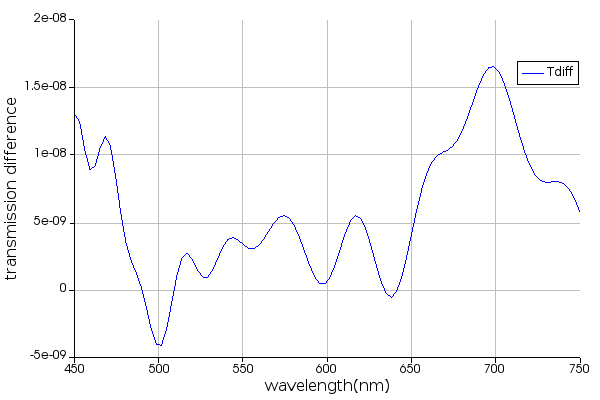
\includegraphics[width=0.75\textwidth]{T_diff_two_polar-s-0-90.png}
    \caption{Difference plot between two orthogonal polarizations (0 and 90 degrees).}
    \label{fig:diff}
\end{figure}

The sweep is set up for the size of the FDTD box (z span). The source and detectors are placed 50 nm inward off the top and bottom edge respectively. Separation between source and monitor does not matter as long as it is more than about 700 nm.  Below this value the auto shut-off level is set to 1 and the simulation terminates prematurely, producing no T result. The separation length more than this value has no effect (Figure~\ref{fig:separation}).

\begin{figure}
    \centering
    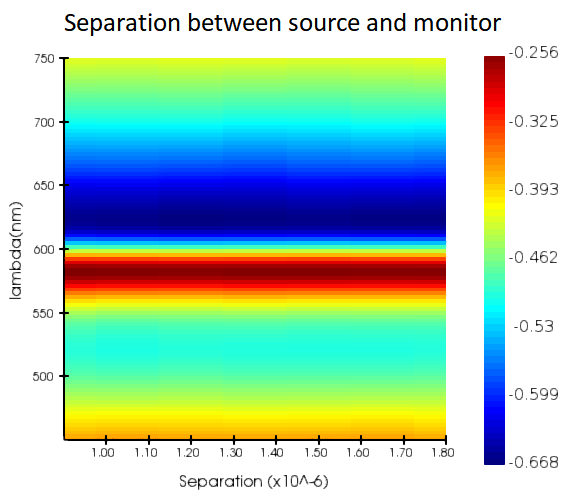
\includegraphics[width=0.75\textwidth]{separation_sweep.png}
    \caption{Sweep data for different separation between source and monitor. Separation (x-axis) refers to ``z span'' of FDTD solver box. The actual distances between the source and monitor are 100 nm less than the corresponding values.}
    \label{fig:separation}
\end{figure}

Meshing accuracy for FDTD was swept for the standard values between 1-8 (Figure~\ref{fig:meshing}). Obviously, setting mesh accuracy past 3 does not affect the result.

\begin{figure}
    \centering
    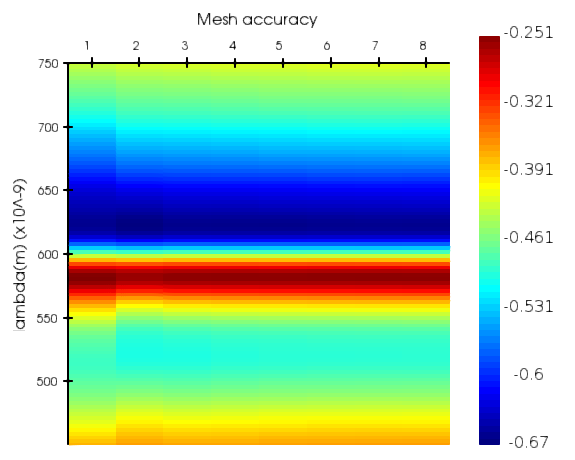
\includegraphics[width=0.75\textwidth]{meshing_accuracy.png}
    \caption{Sweep data for different mesh accuracy in FDTD solver.}
    \label{fig:meshing}
\end{figure}

Mesh override setting (dx, dy and dz simultaneously) was swept for 7 values around reported 4.5 nm, from 1.5 to 7.5 nm (Figure~\ref{fig:override}). While there is certain difference for each value, indeed, 1.5, 4.5, 5.5 and 7.5 nm override produces quite similar results, which justifies the authors' selection.

\begin{figure}
    \centering
    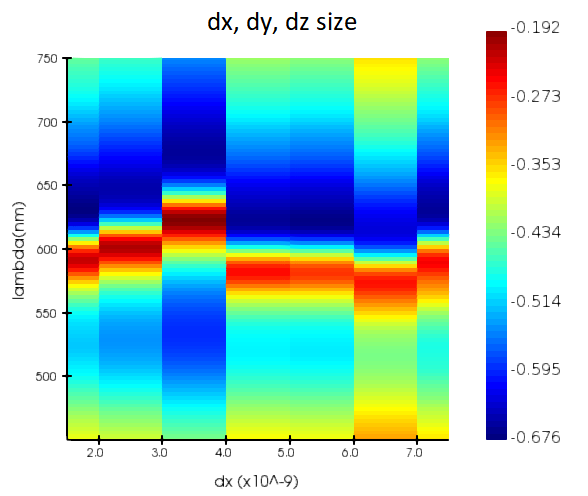
\includegraphics[width=0.75\textwidth]{override_size.png}
    \caption{Sweep data for different mesh override.}
    \label{fig:override}
\end{figure}

Admittedly, setting boundary condition from periodic to symmetric (y) and anti-symmetric (x) for mesh override dx, dy and dz = 1.5 and 4.5 nm provides different results, as well as much longer computation time (20 min against 3 min for 1.5 nm, a few times longer for 4.5 nm). It is logical because the symmetric/anti-symmetric boundary conditions at one end cannot be  combined with periodic conditions at the other end. 



\begin{displayquote}
    \textbf{b.} Reproduce figures 2a, c and e.
\end{displayquote}

The minimum transmission, hence absorbance maximum, was found around 580 nm (pitch 200 nm). To match the resolution, the mesh override was set to 1.5 nm.  
See Figures~\ref{fig:vector},~\ref{fig:efield}~\ref{fig:section}. 

\begin{figure}
    \centering
    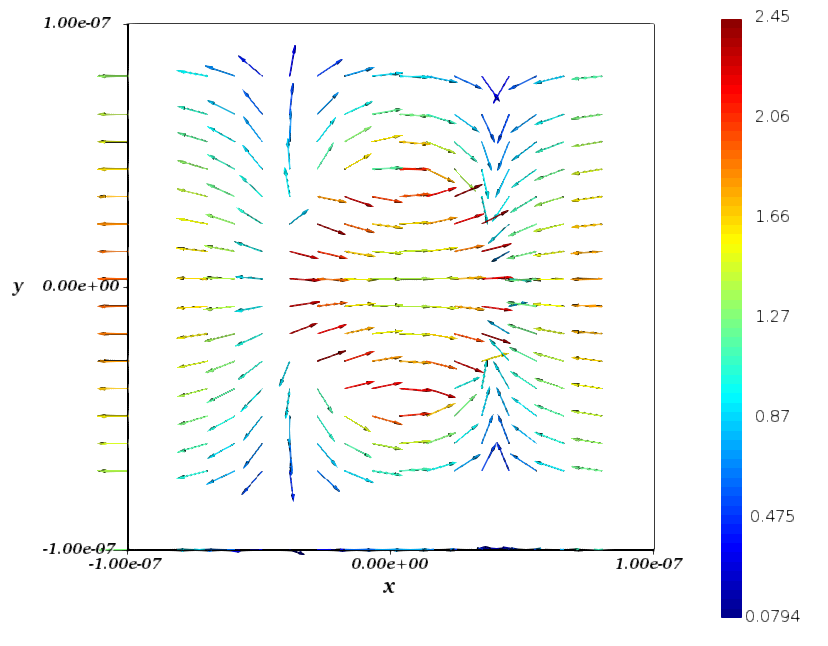
\includegraphics[width=0.75\textwidth]{vector_plot.png}
    \caption{Instantaneous scattered electric  vector field at absorption maximum.}
    \label{fig:vector}
\end{figure}
\begin{figure}
    \centering
    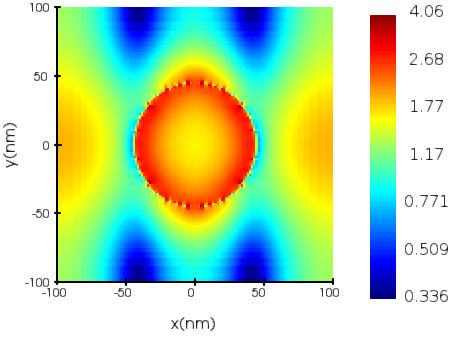
\includegraphics[width=0.75\textwidth]{E-field hole_hires_periodic_BCs.png}
    \caption{Electric field profile at absorption maximum. Intensity pseudo-color is plotted logarithmically to increase contrast.}
    \label{fig:efield}
\end{figure}
\begin{figure}
    \centering
    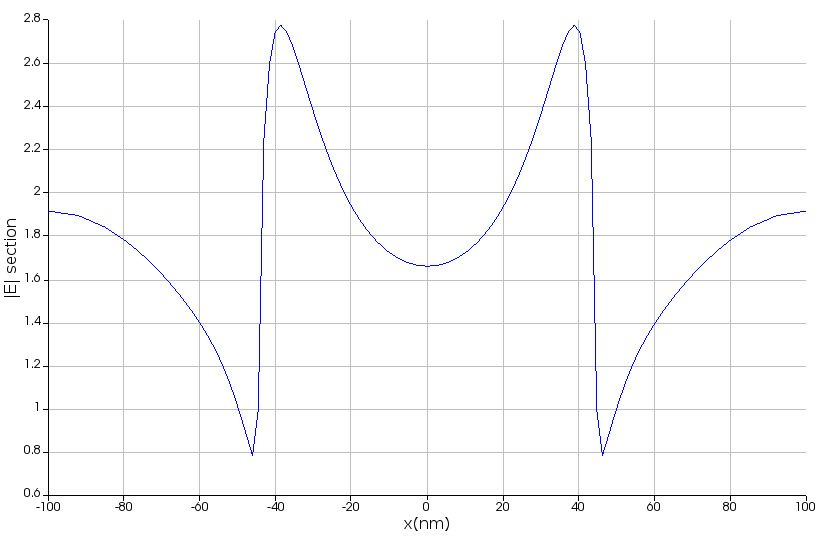
\includegraphics[width=0.75\textwidth]{e-section.png}
    \caption{Electric field (Figure~\ref{fig:efield}) profile of section at $y=0$.}
    \label{fig:section}
\end{figure}

\begin{displayquote}
    \textbf{c.} Reproduce figure 3c. It’s not necessary to get the absolute transmission values right, but the general trends need to be there.
\end{displayquote}

See Figure~\ref{fig:three}. For the purpose of producing this figure, the main script was repeated three times sequentially, with different array periods (\verb|ax, ay|) and the graphs were plotted using \verb|holdon|. 
\begin{figure}
    \centering
    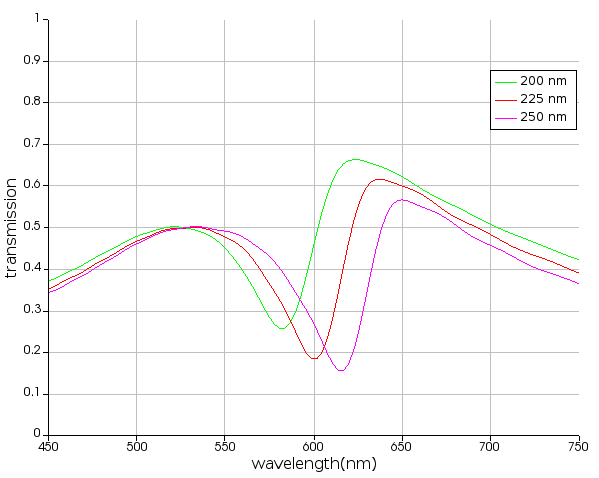
\includegraphics[width=0.75\textwidth]{Three_pitches.png}
    \caption{Simulated transmission spectra for 90 nm diameter hole arrays with periodicity 200, 225, 250 nm.}
    \label{fig:three}
\end{figure}

\begin{displayquote}
    \textbf{d.} Measure the transmittance of the film itself. Use this and the ratio of the hole area to the lattice unit cell to calculate the expected transmission if you knew nothing about wave optics and plasmonics (ballistic transmission through a grid). Comment on how well they match.
\end{displayquote}
Transmission of Au film was recorded using the same model, with the holes disabled (Figure~\ref{fig:aufilm}). For a 200 nm separation, there is approximately 16 percent empty space, while the transmission graph of the plain film almost corresponds to that of the photonic crystal at the ends, it is not trivial to predict the dip in transmission, that is accountable for filtering, as well as larger peak transmission. 

\begin{figure}
    \centering
    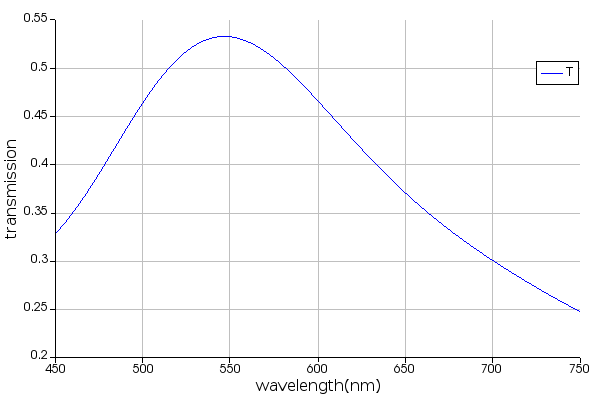
\includegraphics[width=0.75\textwidth]{transmission_of_au_film.png}
    \caption{Simulated transmission spectrum for 20 nm Au film.}
    \label{fig:aufilm}
\end{figure}

\end{document}
